\documentclass[12pt,a4paper]{article}
\usepackage[utf8]{vietnam}
\usepackage{amsmath,amssymb}
\usepackage{tabularx}
\usepackage{tikz}
\usepackage{xcolor}
\usepackage[top=0.6cm, bottom=0.6cm, left=0.6cm, right=0.6cm]{geometry}
\usepackage[dethi]{ex_test}

\SAOPTN{widthSA=2.6,heightSA=0.62}
\setlength{\parskip}{0pt}

% Dong ke cham mo chuan viet tay
\newcommand{\dongke}[1]{%
  \begingroup%
  \setlength{\parskip}{0pt}%
  \baselineskip=18.5pt%
  \vspace{1.0mm}%
  \foreach \i in {1,...,#1}{%
    \noindent{\color{gray!60}\dotfill}\par%
  }%
  \vspace{0.6mm}%
  \endgroup%
}

% Khu vuc bai lam chia 2 cot co vach ngan mo o giua
\newcommand{\dongkeHaiCot}[1]{%
  \par\vspace{0.5mm}%
  \noindent%
  \begin{minipage}[t]{0.485\linewidth}%
    \dongke{#1}%
  \end{minipage}%
  \hfill%
  {\color{gray!60}\vrule}%
  \hfill%
  \begin{minipage}[t]{0.485\linewidth}%
    \dongke{#1}%
  \end{minipage}%
}

% Dinh nghia o bai tap tu luan trong bang
\newcommand{\oBaiTap}[3][5]{%
  \vspace{1.0mm}%
  \noindent\textbf{#2} #3\par%
  \dongke{#1}%
}

\begin{document}
\pagestyle{empty}
% =============================================================================
% ========================= TOAN 7 TUAN 09 BUOI 01 - MA DE 101 =================
% ========================= TRANG 1/2 ==========================================
% =============================================================================
\noindent
\begin{tabularx}{\linewidth}{|X|c|}
\hline
\textbf{PHIẾU KIỂM TRA ĐỊNH KỲ TOÁN 7 - TUẦN 09 - BUỔI 01} & \textbf{Mã đề: 101 - Trang 1/2} \\
\hline
\end{tabularx}

\vspace{1.2mm}

\noindent
\begin{tabularx}{\linewidth}{|p{3.2cm}|X|}
\hline
\centering\textbf{ĐIỂM SỐ} & \centering\textbf{LỜI NHẬN XÉT CỦA THẦY CÔ} \tabularnewline
\hline
\rule{0pt}{1.8cm} & \tabularnewline
\hline
\end{tabularx}

\vspace{1.5mm}
\noindent\textbf{Câu 1 (0,25 điểm).} Số đối của số hữu tỉ $-\dfrac{3}{5}$ là: \shortans{\dfrac{3}{5}}\par\vspace{2.3mm}
\noindent\textbf{Câu 2 (0,25 điểm).} Giá trị của căn bậc hai số học $\sqrt{64}$ bằng: \shortans{8}\par\vspace{2.3mm}
\noindent\textbf{Câu 3 (0,25 điểm).} Giá trị của biểu thức $|-4{,}75|$ bằng: \shortans{4{,}75}\par\vspace{2.3mm}
\noindent\textbf{Câu 4 (0,25 điểm).} Tổng ba góc trong một tam giác bằng bao nhiêu độ? \shortans{180^\circ}\par\vspace{2.3mm}
\noindent\textbf{Câu 5 (0,25 điểm).} Cho $\Delta ABC$ có $\widehat{A} = 65^\circ, \widehat{B} = 55^\circ$. Số đo góc $\widehat{C}$ là: \shortans{60^\circ}\par\vspace{2.3mm}
\noindent\textbf{Câu 6 (0,25 điểm).} Cho $\Delta MNP$ vuông tại $M$, biết $\widehat{N} = 42^\circ$. Số đo góc $\widehat{P}$ là: \shortans{48^\circ}\par\vspace{2.3mm}
\noindent\textbf{Câu 7 (0,25 điểm).} Tam giác có ba góc tỉ lệ với $1 : 2 : 3$. Số đo góc lớn nhất là: \shortans{90^\circ}\par\vspace{2.3mm}
\noindent\textbf{Câu 8 (0,25 điểm).} Tam giác $DEF$ có $\widehat{D} = 105^\circ$. Tam giác $DEF$ là loại tam giác gì? \shortans{\text{Tam giác tù}}\par\vspace{2.3mm}
\noindent\textbf{Câu 9 (0,25 điểm).} Cho $\Delta ABC$ vuông tại $A$, kẻ đường cao $AH$. Biết $\widehat{B} = 50^\circ$. Số đo góc $\widehat{HAC}$ là: \shortans{50^\circ}\par\vspace{2.3mm}
\noindent\textbf{Câu 10 (0,25 điểm).} Một chiếc thang dựa vào tường tạo với mặt đất góc $70^\circ$. Góc giữa thang và tường là: \shortans{20^\circ}\par\vspace{2.3mm}
\vspace{0.2mm}
\noindent\textbf{Câu 11 (3,0 điểm). Thực hiện phép tính (hợp lý nếu có thể):}
\vspace{0.8mm}

\noindent
\begin{tabularx}{\linewidth}{|X|X|}
\hline
\oBaiTap[5]{a) (0,5 điểm)}{$\dfrac{3}{7} + \dfrac{5}{14} - \dfrac{1}{2}$} & 
\oBaiTap[5]{b) (0,5 điểm)}{$\dfrac{4}{9} \cdot \left(-\dfrac{5}{7}\right) + \dfrac{4}{9} \cdot \left(-\dfrac{2}{7}\right)$} \\
\hline
\oBaiTap[5]{c) (0,5 điểm)}{$\left(-\dfrac{1}{2}\right)^3 : \dfrac{1}{4} + \dfrac{3}{4} \cdot 2$} & 
\oBaiTap[5]{d) (0,5 điểm)}{$\sqrt{\dfrac{25}{16}} - \left|-\dfrac{3}{4}\right| + \dfrac{1}{2}$} \\
\hline
\oBaiTap[5]{e) (0,5 điểm)}{$\dfrac{5}{2} - \left[\dfrac{3}{4} + \left(\dfrac{1}{2}\right)^2\right]$} & 
\oBaiTap[5]{f) (0,5 điểm)}{$\dfrac{2^{10} \cdot 9^3}{4^4 \cdot 3^7}$} \\
\hline
\end{tabularx}

\newpage
% =============================================================================
% ========================= TOAN 7 TUAN 09 BUOI 01 - MA DE 101 =================
% ========================= TRANG 2/2 ==========================================
% =============================================================================
\noindent
\begin{tabularx}{\linewidth}{|X|c|}
\hline
\textbf{TOÁN 7 - TUẦN 09 - BUỔI 01} & \textbf{Mã đề: 101 - Trang 2/2} \\
\hline
\end{tabularx}

\vspace{1.5mm}

\noindent\textbf{Câu 12 (2,0 điểm). Tìm số hữu tỉ $x$, biết:}
\vspace{0.8mm}

\noindent
\begin{tabularx}{\linewidth}{|X|X|}
\hline
\oBaiTap[5]{a) (0,5 điểm)}{$x - \dfrac{3}{5} = \dfrac{7}{10}$} & 
\oBaiTap[5]{b) (0,5 điểm)}{$\dfrac{2}{3}x + \dfrac{1}{2} = \dfrac{5}{6}$} \\
\hline
\oBaiTap[5]{c) (0,5 điểm)}{$\left(x - \dfrac{1}{3}\right)^2 = \dfrac{4}{9}$} & 
\oBaiTap[5]{d) (0,5 điểm)}{$\left|2x - \dfrac{1}{2}\right| = \dfrac{3}{2}$} \\
\hline
\end{tabularx}

\vspace{1.5mm}

\noindent
\begin{tabularx}{\linewidth}{|X|}
\hline
\vspace{0.5mm}
\begin{minipage}[t]{0.68\linewidth}
\vspace{0pt}
\textbf{Câu 13 (2,0 điểm).} Cho tam giác $ABC$ vuông tại $A$ ($AB < AC$), biết $\widehat{B} = 60^\circ$. Kẻ đường cao $AH$ ($H \in BC$).\par\vspace{0.4mm}
\textbf{a)} (1,0 điểm) Tính số đo các góc $\widehat{C}$ và $\widehat{HAB}$.\par\vspace{0.4mm}
\textbf{b)} (1,0 điểm) Kẻ tia phân giác của góc $\widehat{HAC}$ cắt cạnh $BC$ tại $D$. Chứng minh rằng tam giác $ABD$ có $\widehat{BAD} = \widehat{BDA}$.
\end{minipage}\hfill
\begin{minipage}[t]{0.30\linewidth}
\vspace{0pt}\centering
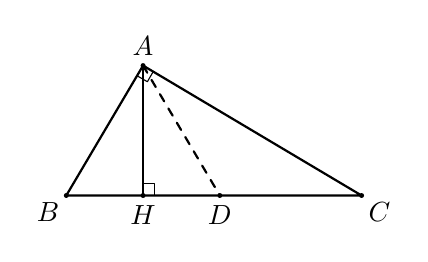
\begin{tikzpicture}[scale=0.75, >=stealth, line join=round, line cap=round]
  \coordinate (H) at (0, 0);
  \coordinate (A) at (0, 2.2);
  \coordinate (B) at (-1.3, 0);
  \coordinate (C) at (3.7, 0);
  \coordinate (D) at (1.3, 0);
  \draw[thick] (B) -- (A) -- (C) -- cycle;
  \draw[thick] (A) -- (H);
  \draw[thick, dashed] (A) -- (D);
  \draw (0, 0.2) -- (0.2, 0.2) -- (0.2, 0);
  \draw[rotate=-30] (A) rectangle +(0.2, -0.2);
  \fill (A) circle (1.2pt) node[above] {$A$};
  \fill (B) circle (1.2pt) node[below left=-1pt] {$B$};
  \fill (C) circle (1.2pt) node[below right=-1pt] {$C$};
  \fill (H) circle (1.2pt) node[below] {$H$};
  \fill (D) circle (1.2pt) node[below] {$D$};
\end{tikzpicture}
\end{minipage}\par
\vspace{0.4mm}
\noindent\textit{Bài giải:}\dongkeHaiCot{11}
\\ \hline
\end{tabularx}

\vspace{1.5mm}

\noindent
\begin{tabularx}{\linewidth}{|X|}
\hline
\vspace{0.5mm}
\textbf{Câu 14 (0,5 điểm).} Tìm giá trị nhỏ nhất của biểu thức: $A = |x - 2026| + |x - 2|$.\par
\vspace{0.4mm}
\noindent\textit{Bài giải:}\dongkeHaiCot{7}
\\ \hline
\end{tabularx}

\newpage
% =============================================================================
% ========================= TOAN 7 TUAN 09 BUOI 01 - MA DE 102 =================
% ========================= TRANG 1/2 ==========================================
% =============================================================================
\noindent
\begin{tabularx}{\linewidth}{|X|c|}
\hline
\textbf{PHIẾU KIỂM TRA ĐỊNH KỲ TOÁN 7 - TUẦN 09 - BUỔI 01} & \textbf{Mã đề: 102 - Trang 1/2} \\
\hline
\end{tabularx}

\vspace{1.2mm}

\noindent
\begin{tabularx}{\linewidth}{|p{3.2cm}|X|}
\hline
\centering\textbf{ĐIỂM SỐ} & \centering\textbf{LỜI NHẬN XÉT CỦA THẦY CÔ} \tabularnewline
\hline
\rule{0pt}{1.8cm} & \tabularnewline
\hline
\end{tabularx}

\vspace{1.5mm}
\noindent\textbf{Câu 1 (0,25 điểm).} Số đối của số hữu tỉ $-\dfrac{4}{9}$ là: \shortans{\dfrac{4}{9}}\par\vspace{2.3mm}
\noindent\textbf{Câu 2 (0,25 điểm).} Giá trị của căn bậc hai số học $\sqrt{49}$ bằng: \shortans{7}\par\vspace{2.3mm}
\noindent\textbf{Câu 3 (0,25 điểm).} Giá trị của biểu thức $|-5{,}25|$ bằng: \shortans{5{,}25}\par\vspace{2.3mm}
\noindent\textbf{Câu 4 (0,25 điểm).} Tổng ba góc trong một tam giác bằng bao nhiêu độ? \shortans{180^\circ}\par\vspace{2.3mm}
\noindent\textbf{Câu 5 (0,25 điểm).} Cho $\Delta ABC$ có $\widehat{A} = 70^\circ, \widehat{B} = 45^\circ$. Số đo góc $\widehat{C}$ là: \shortans{65^\circ}\par\vspace{2.3mm}
\noindent\textbf{Câu 6 (0,25 điểm).} Cho $\Delta MNP$ vuông tại $M$, biết $\widehat{N} = 35^\circ$. Số đo góc $\widehat{P}$ là: \shortans{55^\circ}\par\vspace{2.3mm}
\noindent\textbf{Câu 7 (0,25 điểm).} Tam giác có ba góc tỉ lệ với $2 : 3 : 4$. Số đo góc nhỏ nhất là: \shortans{40^\circ}\par\vspace{2.3mm}
\noindent\textbf{Câu 8 (0,25 điểm).} Tam giác $GHK$ có $\widehat{G} = 95^\circ$. Tam giác $GHK$ là loại tam giác gì? \shortans{\text{Tam giác tù}}\par\vspace{2.3mm}
\noindent\textbf{Câu 9 (0,25 điểm).} Cho $\Delta ABC$ vuông tại $A$, kẻ đường cao $AH$. Biết $\widehat{B} = 55^\circ$. Số đo góc $\widehat{HAC}$ là: \shortans{55^\circ}\par\vspace{2.3mm}
\noindent\textbf{Câu 10 (0,25 điểm).} Một chiếc thang dựa vào tường tạo với mặt đất góc $65^\circ$. Góc giữa thang và tường là: \shortans{25^\circ}\par\vspace{2.3mm}
\vspace{0.2mm}
\noindent\textbf{Câu 11 (3,0 điểm). Thực hiện phép tính (hợp lý nếu có thể):}
\vspace{0.8mm}

\noindent
\begin{tabularx}{\linewidth}{|X|X|}
\hline
\oBaiTap[5]{a) (0,5 điểm)}{$\dfrac{2}{5} + \dfrac{7}{10} - \dfrac{1}{2}$} & 
\oBaiTap[5]{b) (0,5 điểm)}{$\dfrac{5}{8} \cdot \left(-\dfrac{4}{9}\right) + \dfrac{5}{8} \cdot \left(-\dfrac{5}{9}\right)$} \\
\hline
\oBaiTap[5]{c) (0,5 điểm)}{$\left(-\dfrac{1}{3}\right)^2 \cdot 9 - \dfrac{5}{6} : \dfrac{5}{3}$} & 
\oBaiTap[5]{d) (0,5 điểm)}{$\sqrt{\dfrac{36}{25}} - \left|-\dfrac{4}{5}\right| + \dfrac{3}{5}$} \\
\hline
\oBaiTap[5]{e) (0,5 điểm)}{$\dfrac{7}{2} - \left[\dfrac{5}{4} + \left(\dfrac{1}{2}\right)^2\right]$} & 
\oBaiTap[5]{f) (0,5 điểm)}{$\dfrac{3^{10} \cdot 4^3}{9^4 \cdot 2^7}$} \\
\hline
\end{tabularx}

\newpage
% =============================================================================
% ========================= TOAN 7 TUAN 09 BUOI 01 - MA DE 102 =================
% ========================= TRANG 2/2 ==========================================
% =============================================================================
\noindent
\begin{tabularx}{\linewidth}{|X|c|}
\hline
\textbf{TOÁN 7 - TUẦN 09 - BUỔI 01} & \textbf{Mã đề: 102 - Trang 2/2} \\
\hline
\end{tabularx}

\vspace{1.5mm}

\noindent\textbf{Câu 12 (2,0 điểm). Tìm số hữu tỉ $x$, biết:}
\vspace{0.8mm}

\noindent
\begin{tabularx}{\linewidth}{|X|X|}
\hline
\oBaiTap[5]{a) (0,5 điểm)}{$x - \dfrac{2}{3} = \dfrac{5}{6}$} & 
\oBaiTap[5]{b) (0,5 điểm)}{$\dfrac{3}{4}x + \dfrac{1}{3} = \dfrac{7}{12}$} \\
\hline
\oBaiTap[5]{c) (0,5 điểm)}{$\left(x - \dfrac{1}{2}\right)^2 = \dfrac{9}{16}$} & 
\oBaiTap[5]{d) (0,5 điểm)}{$\left|3x - \dfrac{1}{3}\right| = \dfrac{5}{3}$} \\
\hline
\end{tabularx}

\vspace{1.5mm}

\noindent
\begin{tabularx}{\linewidth}{|X|}
\hline
\vspace{0.5mm}
\begin{minipage}[t]{0.68\linewidth}
\vspace{0pt}
\textbf{Câu 13 (2,0 điểm).} Cho tam giác $ABC$ vuông tại $A$ ($AB < AC$), biết $\widehat{B} = 50^\circ$. Kẻ đường cao $AH$ ($H \in BC$).\par\vspace{0.4mm}
\textbf{a)} (1,0 điểm) Tính số đo các góc $\widehat{C}$ và $\widehat{HAB}$.\par\vspace{0.4mm}
\textbf{b)} (1,0 điểm) Kẻ tia phân giác của góc $\widehat{HAC}$ cắt cạnh $BC$ tại $D$. Chứng minh rằng tam giác $ABD$ có $\widehat{BAD} = \widehat{BDA}$.
\end{minipage}\hfill
\begin{minipage}[t]{0.30\linewidth}
\vspace{0pt}\centering
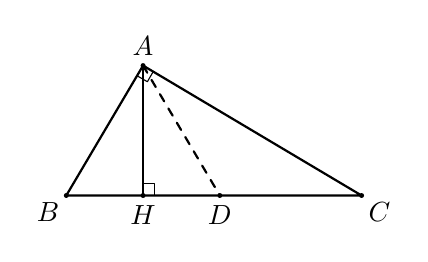
\begin{tikzpicture}[scale=0.75, >=stealth, line join=round, line cap=round]
  \coordinate (H) at (0, 0);
  \coordinate (A) at (0, 2.2);
  \coordinate (B) at (-1.3, 0);
  \coordinate (C) at (3.7, 0);
  \coordinate (D) at (1.3, 0);
  \draw[thick] (B) -- (A) -- (C) -- cycle;
  \draw[thick] (A) -- (H);
  \draw[thick, dashed] (A) -- (D);
  \draw (0, 0.2) -- (0.2, 0.2) -- (0.2, 0);
  \draw[rotate=-30] (A) rectangle +(0.2, -0.2);
  \fill (A) circle (1.2pt) node[above] {$A$};
  \fill (B) circle (1.2pt) node[below left=-1pt] {$B$};
  \fill (C) circle (1.2pt) node[below right=-1pt] {$C$};
  \fill (H) circle (1.2pt) node[below] {$H$};
  \fill (D) circle (1.2pt) node[below] {$D$};
\end{tikzpicture}
\end{minipage}\par
\vspace{0.4mm}
\noindent\textit{Bài giải:}\dongkeHaiCot{11}
\\ \hline
\end{tabularx}

\vspace{1.5mm}

\noindent
\begin{tabularx}{\linewidth}{|X|}
\hline
\vspace{0.5mm}
\textbf{Câu 14 (0,5 điểm).} Tìm giá trị nhỏ nhất của biểu thức: $A = |x - 2025| + |x - 3|$.\par
\vspace{0.4mm}
\noindent\textit{Bài giải:}\dongkeHaiCot{7}
\\ \hline
\end{tabularx}

\newpage
% =============================================================================
% ========================= TOAN 7 TUAN 09 BUOI 01 - MA DE 103 =================
% ========================= TRANG 1/2 ==========================================
% =============================================================================
\noindent
\begin{tabularx}{\linewidth}{|X|c|}
\hline
\textbf{PHIẾU KIỂM TRA ĐỊNH KỲ TOÁN 7 - TUẦN 09 - BUỔI 01} & \textbf{Mã đề: 103 - Trang 1/2} \\
\hline
\end{tabularx}

\vspace{1.2mm}

\noindent
\begin{tabularx}{\linewidth}{|p{3.2cm}|X|}
\hline
\centering\textbf{ĐIỂM SỐ} & \centering\textbf{LỜI NHẬN XÉT CỦA THẦY CÔ} \tabularnewline
\hline
\rule{0pt}{1.8cm} & \tabularnewline
\hline
\end{tabularx}

\vspace{1.5mm}
\noindent\textbf{Câu 1 (0,25 điểm).} Số đối của số hữu tỉ $-\dfrac{5}{8}$ là: \shortans{\dfrac{5}{8}}\par\vspace{2.3mm}
\noindent\textbf{Câu 2 (0,25 điểm).} Giá trị của căn bậc hai số học $\sqrt{100}$ bằng: \shortans{10}\par\vspace{2.3mm}
\noindent\textbf{Câu 3 (0,25 điểm).} Giá trị của biểu thức $|-3{,}85|$ bằng: \shortans{3{,}85}\par\vspace{2.3mm}
\noindent\textbf{Câu 4 (0,25 điểm).} Tổng ba góc trong một tam giác bằng bao nhiêu độ? \shortans{180^\circ}\par\vspace{2.3mm}
\noindent\textbf{Câu 5 (0,25 điểm).} Cho $\Delta ABC$ có $\widehat{A} = 80^\circ, \widehat{B} = 40^\circ$. Số đo góc $\widehat{C}$ là: \shortans{60^\circ}\par\vspace{2.3mm}
\noindent\textbf{Câu 6 (0,25 điểm).} Cho $\Delta MNP$ vuông tại $M$, biết $\widehat{N} = 52^\circ$. Số đo góc $\widehat{P}$ là: \shortans{38^\circ}\par\vspace{2.3mm}
\noindent\textbf{Câu 7 (0,25 điểm).} Tam giác có ba góc tỉ lệ với $1 : 3 : 5$. Số đo góc lớn nhất là: \shortans{100^\circ}\par\vspace{2.3mm}
\noindent\textbf{Câu 8 (0,25 điểm).} Tam giác $PQR$ có $\widehat{P} = 100^\circ$. Tam giác $PQR$ là loại tam giác gì? \shortans{\text{Tam giác tù}}\par\vspace{2.3mm}
\noindent\textbf{Câu 9 (0,25 điểm).} Cho $\Delta ABC$ vuông tại $A$, kẻ đường cao $AH$. Biết $\widehat{B} = 40^\circ$. Số đo góc $\widehat{HAC}$ là: \shortans{40^\circ}\par\vspace{2.3mm}
\noindent\textbf{Câu 10 (0,25 điểm).} Một chiếc thang dựa vào tường tạo với mặt đất góc $75^\circ$. Góc giữa thang và tường là: \shortans{15^\circ}\par\vspace{2.3mm}
\vspace{0.2mm}
\noindent\textbf{Câu 11 (3,0 điểm). Thực hiện phép tính (hợp lý nếu có thể):}
\vspace{0.8mm}

\noindent
\begin{tabularx}{\linewidth}{|X|X|}
\hline
\oBaiTap[5]{a) (0,5 điểm)}{$\dfrac{4}{9} + \dfrac{5}{18} - \dfrac{1}{3}$} & 
\oBaiTap[5]{b) (0,5 điểm)}{$\dfrac{3}{7} \cdot \left(-\dfrac{5}{11}\right) + \dfrac{3}{7} \cdot \left(-\dfrac{6}{11}\right)$} \\
\hline
\oBaiTap[5]{c) (0,5 điểm)}{$\left(-\dfrac{1}{2}\right)^4 \cdot 16 + \dfrac{2}{3} : \dfrac{4}{9}$} & 
\oBaiTap[5]{d) (0,5 điểm)}{$\sqrt{\dfrac{49}{36}} - \left|-\dfrac{5}{6}\right| + \dfrac{2}{3}$} \\
\hline
\oBaiTap[5]{e) (0,5 điểm)}{$\dfrac{9}{2} - \left[\dfrac{7}{4} + \left(\dfrac{1}{2}\right)^2\right]$} & 
\oBaiTap[5]{f) (0,5 điểm)}{$\dfrac{2^9 \cdot 25^2}{10^4 \cdot 4}$} \\
\hline
\end{tabularx}

\newpage
% =============================================================================
% ========================= TOAN 7 TUAN 09 BUOI 01 - MA DE 103 =================
% ========================= TRANG 2/2 ==========================================
% =============================================================================
\noindent
\begin{tabularx}{\linewidth}{|X|c|}
\hline
\textbf{TOÁN 7 - TUẦN 09 - BUỔI 01} & \textbf{Mã đề: 103 - Trang 2/2} \\
\hline
\end{tabularx}

\vspace{1.5mm}

\noindent\textbf{Câu 12 (2,0 điểm). Tìm số hữu tỉ $x$, biết:}
\vspace{0.8mm}

\noindent
\begin{tabularx}{\linewidth}{|X|X|}
\hline
\oBaiTap[5]{a) (0,5 điểm)}{$x - \dfrac{4}{5} = \dfrac{3}{10}$} & 
\oBaiTap[5]{b) (0,5 điểm)}{$\dfrac{4}{5}x + \dfrac{1}{2} = \dfrac{9}{10}$} \\
\hline
\oBaiTap[5]{c) (0,5 điểm)}{$\left(x - \dfrac{1}{4}\right)^2 = \dfrac{9}{16}$} & 
\oBaiTap[5]{d) (0,5 điểm)}{$\left|2x - \dfrac{1}{3}\right| = \dfrac{5}{3}$} \\
\hline
\end{tabularx}

\vspace{1.5mm}

\noindent
\begin{tabularx}{\linewidth}{|X|}
\hline
\vspace{0.5mm}
\begin{minipage}[t]{0.68\linewidth}
\vspace{0pt}
\textbf{Câu 13 (2,0 điểm).} Cho tam giác $ABC$ vuông tại $A$ ($AB < AC$), biết $\widehat{B} = 54^\circ$. Kẻ đường cao $AH$ ($H \in BC$).\par\vspace{0.4mm}
\textbf{a)} (1,0 điểm) Tính số đo các góc $\widehat{C}$ và $\widehat{HAB}$.\par\vspace{0.4mm}
\textbf{b)} (1,0 điểm) Kẻ tia phân giác của góc $\widehat{HAC}$ cắt cạnh $BC$ tại $D$. Chứng minh rằng tam giác $ABD$ có $\widehat{BAD} = \widehat{BDA}$.
\end{minipage}\hfill
\begin{minipage}[t]{0.30\linewidth}
\vspace{0pt}\centering
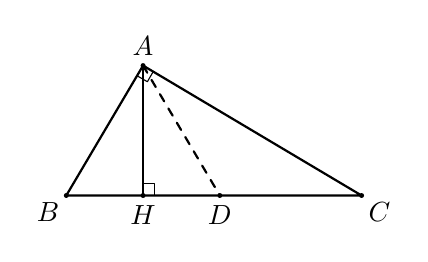
\begin{tikzpicture}[scale=0.75, >=stealth, line join=round, line cap=round]
  \coordinate (H) at (0, 0);
  \coordinate (A) at (0, 2.2);
  \coordinate (B) at (-1.3, 0);
  \coordinate (C) at (3.7, 0);
  \coordinate (D) at (1.3, 0);
  \draw[thick] (B) -- (A) -- (C) -- cycle;
  \draw[thick] (A) -- (H);
  \draw[thick, dashed] (A) -- (D);
  \draw (0, 0.2) -- (0.2, 0.2) -- (0.2, 0);
  \draw[rotate=-30] (A) rectangle +(0.2, -0.2);
  \fill (A) circle (1.2pt) node[above] {$A$};
  \fill (B) circle (1.2pt) node[below left=-1pt] {$B$};
  \fill (C) circle (1.2pt) node[below right=-1pt] {$C$};
  \fill (H) circle (1.2pt) node[below] {$H$};
  \fill (D) circle (1.2pt) node[below] {$D$};
\end{tikzpicture}
\end{minipage}\par
\vspace{0.4mm}
\noindent\textit{Bài giải:}\dongkeHaiCot{11}
\\ \hline
\end{tabularx}

\vspace{1.5mm}

\noindent
\begin{tabularx}{\linewidth}{|X|}
\hline
\vspace{0.5mm}
\textbf{Câu 14 (0,5 điểm).} Tìm giá trị nhỏ nhất của biểu thức: $A = |x - 2024| + |x - 4|$.\par
\vspace{0.4mm}
\noindent\textit{Bài giải:}\dongkeHaiCot{7}
\\ \hline
\end{tabularx}

\newpage
% =============================================================================
% ========================= TOAN 7 TUAN 09 BUOI 01 - MA DE 104 =================
% ========================= TRANG 1/2 ==========================================
% =============================================================================
\noindent
\begin{tabularx}{\linewidth}{|X|c|}
\hline
\textbf{PHIẾU KIỂM TRA ĐỊNH KỲ TOÁN 7 - TUẦN 09 - BUỔI 01} & \textbf{Mã đề: 104 - Trang 1/2} \\
\hline
\end{tabularx}

\vspace{1.2mm}

\noindent
\begin{tabularx}{\linewidth}{|p{3.2cm}|X|}
\hline
\centering\textbf{ĐIỂM SỐ} & \centering\textbf{LỜI NHẬN XÉT CỦA THẦY CÔ} \tabularnewline
\hline
\rule{0pt}{1.8cm} & \tabularnewline
\hline
\end{tabularx}

\vspace{1.5mm}
\noindent\textbf{Câu 1 (0,25 điểm).} Số đối của số hữu tỉ $-\dfrac{5}{6}$ là: \shortans{\dfrac{5}{6}}\par\vspace{2.3mm}
\noindent\textbf{Câu 2 (0,25 điểm).} Giá trị của căn bậc hai số học $\sqrt{121}$ bằng: \shortans{11}\par\vspace{2.3mm}
\noindent\textbf{Câu 3 (0,25 điểm).} Giá trị của biểu thức $|-7{,}15|$ bằng: \shortans{7{,}15}\par\vspace{2.3mm}
\noindent\textbf{Câu 4 (0,25 điểm).} Tổng ba góc trong một tam giác bằng bao nhiêu độ? \shortans{180^\circ}\par\vspace{2.3mm}
\noindent\textbf{Câu 5 (0,25 điểm).} Cho $\Delta ABC$ có $\widehat{A} = 75^\circ, \widehat{B} = 35^\circ$. Số đo góc $\widehat{C}$ là: \shortans{70^\circ}\par\vspace{2.3mm}
\noindent\textbf{Câu 6 (0,25 điểm).} Cho $\Delta MNP$ vuông tại $M$, biết $\widehat{N} = 48^\circ$. Số đo góc $\widehat{P}$ là: \shortans{42^\circ}\par\vspace{2.3mm}
\noindent\textbf{Câu 7 (0,25 điểm).} Tam giác có ba góc tỉ lệ với $2 : 3 : 5$. Số đo góc lớn nhất là: \shortans{90^\circ}\par\vspace{2.3mm}
\noindent\textbf{Câu 8 (0,25 điểm).} Tam giác $XYZ$ có $\widehat{X} = 115^\circ$. Tam giác $XYZ$ là loại tam giác gì? \shortans{\text{Tam giác tù}}\par\vspace{2.3mm}
\noindent\textbf{Câu 9 (0,25 điểm).} Cho $\Delta ABC$ vuông tại $A$, kẻ đường cao $AH$. Biết $\widehat{B} = 65^\circ$. Số đo góc $\widehat{HAC}$ là: \shortans{65^\circ}\par\vspace{2.3mm}
\noindent\textbf{Câu 10 (0,25 điểm).} Một chiếc thang dựa vào tường tạo với mặt đất góc $60^\circ$. Góc giữa thang và tường là: \shortans{30^\circ}\par\vspace{2.3mm}
\vspace{0.2mm}
\noindent\textbf{Câu 11 (3,0 điểm). Thực hiện phép tính (hợp lý nếu có thể):}
\vspace{0.8mm}

\noindent
\begin{tabularx}{\linewidth}{|X|X|}
\hline
\oBaiTap[5]{a) (0,5 điểm)}{$\dfrac{5}{12} + \dfrac{7}{24} - \dfrac{1}{4}$} & 
\oBaiTap[5]{b) (0,5 điểm)}{$\dfrac{6}{11} \cdot \left(-\dfrac{7}{13}\right) + \dfrac{6}{11} \cdot \left(-\dfrac{6}{13}\right)$} \\
\hline
\oBaiTap[5]{c) (0,5 điểm)}{$\left(-\dfrac{1}{3}\right)^3 \cdot 27 + \dfrac{3}{5} : \dfrac{3}{10}$} & 
\oBaiTap[5]{d) (0,5 điểm)}{$\sqrt{\dfrac{81}{49}} - \left|-\dfrac{5}{7}
ight| + \dfrac{3}{7}$} \\
\hline
\oBaiTap[5]{e) (0,5 điểm)}{$\dfrac{11}{2} - \left[\dfrac{9}{4} + \left(\dfrac{1}{2}\right)^2\right]$} & 
\oBaiTap[5]{f) (0,5 điểm)}{$\dfrac{5^8 \cdot 6^3}{15^3 \cdot 25^2}$} \\
\hline
\end{tabularx}

\newpage
% =============================================================================
% ========================= TOAN 7 TUAN 09 BUOI 01 - MA DE 104 =================
% ========================= TRANG 2/2 ==========================================
% =============================================================================
\noindent
\begin{tabularx}{\linewidth}{|X|c|}
\hline
\textbf{TOÁN 7 - TUẦN 09 - BUỔI 01} & \textbf{Mã đề: 104 - Trang 2/2} \\
\hline
\end{tabularx}

\vspace{1.5mm}

\noindent\textbf{Câu 12 (2,0 điểm). Tìm số hữu tỉ $x$, biết:}
\vspace{0.8mm}

\noindent
\begin{tabularx}{\linewidth}{|X|X|}
\hline
\oBaiTap[5]{a) (0,5 điểm)}{$x - \dfrac{5}{6} = \dfrac{7}{12}$} & 
\oBaiTap[5]{b) (0,5 điểm)}{$\dfrac{5}{6}x + \dfrac{1}{4} = \dfrac{3}{4}$} \\
\hline
\oBaiTap[5]{c) (0,5 điểm)}{$\left(x - \dfrac{1}{5}\right)^2 = \dfrac{4}{25}$} & 
\oBaiTap[5]{d) (0,5 điểm)}{$\left|3x - \dfrac{1}{2}\right| = \dfrac{5}{2}$} \\
\hline
\end{tabularx}

\vspace{1.5mm}

\noindent
\begin{tabularx}{\linewidth}{|X|}
\hline
\vspace{0.5mm}
\begin{minipage}[t]{0.68\linewidth}
\vspace{0pt}
\textbf{Câu 13 (2,0 điểm).} Cho tam giác $ABC$ vuông tại $A$ ($AB < AC$), biết $\widehat{B} = 64^\circ$. Kẻ đường cao $AH$ ($H \in BC$).\par\vspace{0.4mm}
\textbf{a)} (1,0 điểm) Tính số đo các góc $\widehat{C}$ và $\widehat{HAB}$.\par\vspace{0.4mm}
\textbf{b)} (1,0 điểm) Kẻ tia phân giác của góc $\widehat{HAC}$ cắt cạnh $BC$ tại $D$. Chứng minh rằng tam giác $ABD$ có $\widehat{BAD} = \widehat{BDA}$.
\end{minipage}\hfill
\begin{minipage}[t]{0.30\linewidth}
\vspace{0pt}\centering
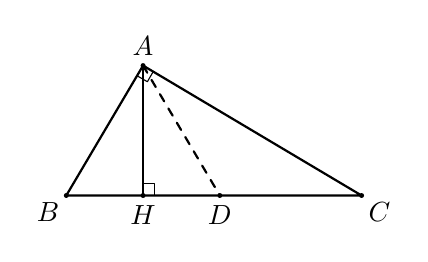
\begin{tikzpicture}[scale=0.75, >=stealth, line join=round, line cap=round]
  \coordinate (H) at (0, 0);
  \coordinate (A) at (0, 2.2);
  \coordinate (B) at (-1.3, 0);
  \coordinate (C) at (3.7, 0);
  \coordinate (D) at (1.3, 0);
  \draw[thick] (B) -- (A) -- (C) -- cycle;
  \draw[thick] (A) -- (H);
  \draw[thick, dashed] (A) -- (D);
  \draw (0, 0.2) -- (0.2, 0.2) -- (0.2, 0);
  \draw[rotate=-30] (A) rectangle +(0.2, -0.2);
  \fill (A) circle (1.2pt) node[above] {$A$};
  \fill (B) circle (1.2pt) node[below left=-1pt] {$B$};
  \fill (C) circle (1.2pt) node[below right=-1pt] {$C$};
  \fill (H) circle (1.2pt) node[below] {$H$};
  \fill (D) circle (1.2pt) node[below] {$D$};
\end{tikzpicture}
\end{minipage}\par
\vspace{0.4mm}
\noindent\textit{Bài giải:}\dongkeHaiCot{11}
\\ \hline
\end{tabularx}

\vspace{1.5mm}

\noindent
\begin{tabularx}{\linewidth}{|X|}
\hline
\vspace{0.5mm}
\textbf{Câu 14 (0,5 điểm).} Tìm giá trị nhỏ nhất của biểu thức: $A = |x - 2023| + |x - 5|$.\par
\vspace{0.4mm}
\noindent\textit{Bài giải:}\dongkeHaiCot{7}
\\ \hline
\end{tabularx}
\end{document}
